% Four composable cost levers feeding one bill, over the "context is compute" base — for Ch25
% ("Cost: The Economics of Running Agents"). Standalone TikZ; compiled by `book-scaffold
% build-figures` via pdflatex -> pdftocairo -> SVG.
% Base = "context is compute" (input context is the spend). Four levers STACK onto it, not compete:
% (1) reduce input context (the driver), (2) prompt caching (write ~1.25x / read ~0.1x),
% (3) model-tier routing (Haiku < Sonnet < Opus, qualitative), (4) Batch API (50% discount).
% NO dollar figures anywhere — ratios and qualitative ordering only.
\documentclass[tikz,border=4mm]{standalone}
\usepackage{tikz}
\usetikzlibrary{positioning, arrows.meta, calc}

\begin{document}
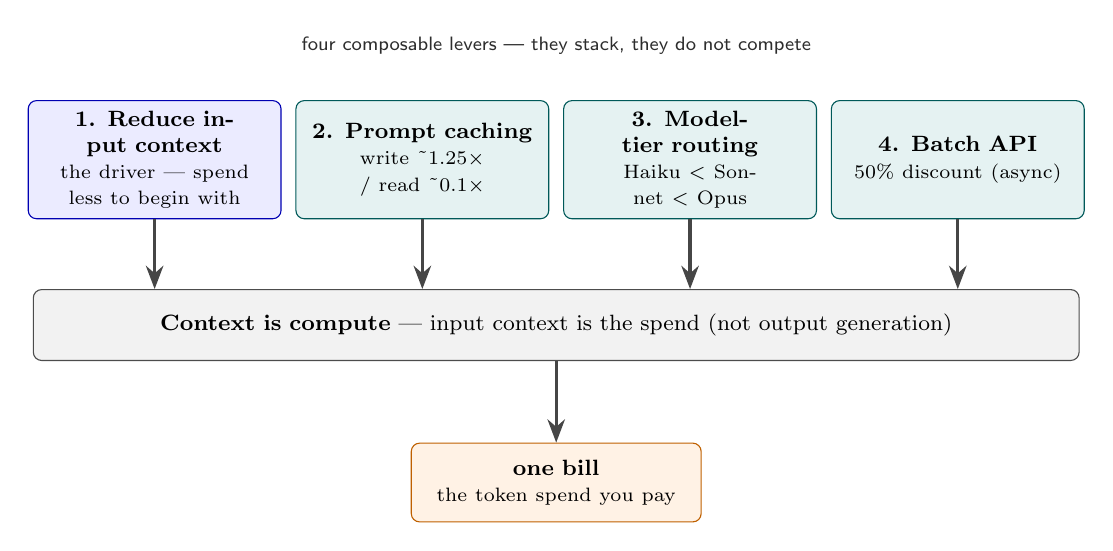
\begin{tikzpicture}[
  font=\sffamily,
  lever/.style={draw=teal!70!black, fill=teal!10, rounded corners=3pt, align=center,
    text width=3.0cm, minimum height=1.5cm, inner sep=3pt, font=\footnotesize},
  driver/.style={draw=blue!70!black, fill=blue!8, rounded corners=3pt, align=center,
    text width=3.0cm, minimum height=1.5cm, inner sep=3pt, font=\footnotesize},
  base/.style={draw=gray!60!black, fill=gray!10, rounded corners=3pt, align=center,
    text width=13.0cm, minimum height=0.9cm, inner sep=4pt, font=\footnotesize},
  bill/.style={draw=orange!75!black, fill=orange!10, rounded corners=3pt, align=center,
    text width=3.4cm, minimum height=1.0cm, inner sep=4pt, font=\footnotesize},
  flow/.style={-Stealth, very thick, draw=gray!55!black},
  note/.style={font=\sffamily\scriptsize, text=gray!35!black}
]

% --- the "context is compute" base ---
\node[base] (base) at (0,0)
  {\textbf{Context is compute} --- input context is the spend (not output generation)};

% --- four composable levers, left to right, sitting ON the base ---
\node[driver] (l1) at (-5.1,2.1)
  {\textbf{1. Reduce input context}\\{\scriptsize the driver --- spend less to begin with}};
\node[lever]  (l2) at (-1.7,2.1)
  {\textbf{2. Prompt caching}\\{\scriptsize write \textasciitilde1.25$\times$ / read \textasciitilde0.1$\times$}};
\node[lever]  (l3) at (1.7,2.1)
  {\textbf{3. Model-tier routing}\\{\scriptsize Haiku $<$ Sonnet $<$ Opus}};
\node[lever]  (l4) at (5.1,2.1)
  {\textbf{4. Batch API}\\{\scriptsize 50\% discount (async)}};

% levers stack onto the base (composable, not competing)
\draw[flow] (l1.south) -- (l1.south |- base.north);
\draw[flow] (l2.south) -- (l2.south |- base.north);
\draw[flow] (l3.south) -- (l3.south |- base.north);
\draw[flow] (l4.south) -- (l4.south |- base.north);

\node[note] at (0,3.55) {four composable levers --- they stack, they do not compete};

% --- the base feeds one bill ---
\node[bill] (bill) at (0,-2.0) {\textbf{one bill}\\{\scriptsize the token spend you pay}};
\draw[flow] (base.south) -- (bill.north);

\end{tikzpicture}
\end{document}
